\documentclass{article}
\usepackage{lmodern}
\usepackage[T1]{fontenc}
\usepackage[english,activeacute]{babel}
\usepackage{mathtools}
\usepackage{biblatex}
\usepackage{csquotes}
\usepackage{graphicx}
\usepackage[]{algorithm2e}
\usepackage[table,xcdraw]{xcolor}
 \usepackage{booktabs}

%\setcounter{tocdepth}{5}
\setcounter{secnumdepth}{5}

\title{User Behavior Analysis in Campus Area Networks through Kohonen Self Organizing Feature Maps}

\author{Nelson Victor Cruz Hern\'andez }

\date{June 2017}

\begin{document}

\maketitle






\section{Introduction} % level 1




\subsection{Background} % level 2
En base al reporte de seguridad de Cisco publicado en 2015 [1] los usuarios y los equipos de Tecnolog�as de informaci�n se han vuelto clave en la seguridad inform�tica dado que estos comprometen la seguridad de forma inconsciente a trav�s del uso indiscriminado de los navegadores y la participaci�n en campa�as de publicidad [1], principales medios para la distribuci�n de malware.

Las t�cnicas actuales de seguridad en redes de computadoras trabajan principalmente en la frontera de la red, buscando prevenir los ataques que son ejecutados desde el exterior descuidando en mayor forma las amenazas que se originan en el interior. 

Se han desarrollados diversos trabajos buscando prevenir y contener los ataques por parte de usuarios internos con diferentes propuestas como son; t�cnicas de Machine Learning y Sistemas de Detecci�n de Intrusos (IDS por sus siglas en ingl�s) [2] [3], algoritmos de clustering [2, 4, 5], generaci�n de infraestructuras de cloud computing y miner�a de datos [4]. 
Dentro de las propuestas de nuevas t�cnicas de IDS existe la problem�tica de los altos �ndices de falsos positivos, una tasa de detecci�n que var�a en base al tipo de ataque, y una dependencia completa a la creaci�n de firmas que muchas veces pueden nos ser optimas en el ambiente de producci�n o sus tiempo de creaci�n es demasiado largo, siendo las principales razones de esto la extensa cantidad de informaci�n que debe ser analizada, el poco tiempo que se tiene para su an�lisis, el uso incorrecto de las t�cnicas de procesamiento aplicadas o el tiempo que se debe invertir para la creaci�n de firmas para el ambiente vulnerable.

Tian [3] propone que es posible hacer uso de selecci�n de variables, para  reducir el conjunto de informaci�n a analizar lo que impacta directamente en el tiempo que se toma el an�lisis y es posible analizar de forma m�s detallada la informaci�n. Por su parte Kamarularin [2] explora la eficiencia de los procesos.

Por su lado Yamada [5] y Kamarularin [2] ejecutan diferentes algoritmos de machine learning cuyos resultados permitan conocer y comparar resultados en la detecci�n de ataques y la retroalimentaci�n para la generaci�n de firmas de forma automatizada.

Es posible observar que existe un campo de estudio enfocado a los IDS, utilizando t�cnicas de machine learning con un alto nivel fiabilidad, por lo que su aplicaci�n permitir�a combatir de forma efectiva la brecha de seguridad en redes causada por los mismos usuarios




\subsection{Justification} % level 2
Current security network solutions neglect  the internal monitoring of users activity, as they assume that inner user interaction is secure and will not harm any asset of the network [10]. However the lack of supervision and monitoring arise two new kind of network vulnerabilities: 1) an inner user attacks the network with full knowledge of what he is doing, while in the other hand 2) an inner user, is victim of an attacker, unconsciently causing attacks to the network, or networks, where it is has any activity. In both scenarios, the user is taking advantage of its unsupervised position.

In the first case, when the user is aware of its not authorized actions, its possible to find two different profiles: 1) basic users and 2) intermediate-advance users [REFERENCE].
Basic malicious users are forced to explode known system vulnerabilities, depending on missing security patches in the operating systems and to use code (snippets and scripts) written by experienced users, as they have a lack of technical formation, making its network behavior similar to a \textit{scriptkiddie}. On the other hand, intermediate-advance users may use new specialized software or tools to break into the network and damage valuable information.

In the case where the host has been compromised and it's being used to generate an attack, both previously explained behaviors can be detected over the network [REFERENCE].

As normal inner users and anomalous users interact in the same network, characterization of both behaviors can provide the required information to detect anomalous users.

\subsection{Problem} % level 2
Identifying network attacks has been addressed in two different ways: 1) Using Signature Based Intrusion Detection Systems (IDS), in which the firms of known attacks are provided to security network devices such as firewalls, antivirus or intrusion detection systems to check if the current network traffic matches any of them the other case are 2) Anomalies-based Intrusion Detection Systems, that make use of artificial intelligence or machine learning algorithms to detect anomalous behavior.

In Signature Based IDS, network devices are able to detect anomalous behavior that completely matches any of the firms in the known attacks database (KAD), missing by far, corner cases such as variations, or improvements of the same attack. Besides this, novel attacks are completely ignored as they do not match any firm in KAD. Both scenarios make keeping up with security updates tedious, time consuming and expensive.

In Anomalies-based IDS, in order to avoid firms classification which implies spending time and human resources, firms are obtained from general datasets such as KDCUPP99 [29-32], causing a big rate of false-positives, making the system not as reliable as it should be.

Attack firms usage is not a viable solution because its process of creation takes a lot of time, experienced human resources are limited or expensive, and software updates are not always available due they do not exist or are expensive.

\subsection{Hypothesis} % level 2
As we form our own criteria, our environment, actions and thoughts start to model how we behave and respond to different stimulus in our day to day situations, in the same way, with the usage of internet in every aspect of our life, a network behavior pattern could be obtained from our digital interaction.

In this work, we state that an user has a defined behavior and that this behavior is constant over time, being able to model it as pattern, based on user's network traffic.

\subsection{Objectives} % level 2
\subsubsection{General Objectives} % level 3
As explained on sections 1.2 and 1.3, there's an obvious need to improve current network security tools, addressing as many problems as possible to solve. By the time this work is being done, we believe that identifying network attacks could be much easier if the amount of variables is reduced from the equation. The actual network security systems deal with normal and anomalous traffic inside and outside the network; but we cannot control what happens outside the frontiers of our network, although we can control what happens inside ours, and define what is a normal behavior in our environment.

The daily interactions of our users will define what is a normal behaviour inside the network, maybe on an ethical \textit{hacker} consultancy, or a security class, network attacks will be common and normal, but this will not be the situation in a house network or in the human resources department. To define what is normal in our environment is vital.
Being able to identify individually any user in our network is a path to identify what is the normal behavior of that user, so that when an attack is performed intentionally or unconsciously users behavior will change and not match to what we previously define as normal.

In this work we demonstrate that it is possible to identify a network user, with a high rate detection, based on it's processed network traffic, and that it is possible to differentiate it from the other users in the same network.

\subsubsection{Particular Objectives} % level 3
User characterization will be done through the creation of an user network pattern, this pattern will be created by a non-supervised clustering algorithm.

This work, address to cover 1) user characterization and 2) project scalability and maintainability.

\paragraph{User characterization} % level 4
A Kohonen Self-organizing map (SOM) algorithm was chosen as the clustering algorithm, due its characteristics of non supervised training, and easy implementation. Trained SOM will allow to identify users inside the network by matching their top features.

\paragraph{Project scalability and maintainability} % level 4
An advantage of the SOM algorithm is that it does not need specific labeled dataset for training or evaluation, adding new users or departments to the organization is as easy as adding what the hosts are transmitting in the correct format. Such tasks will be automated and do not need the supervision of the network administrator.

\section{State of Art} % level 1
With the explosive growth of the internet in the past two decades and the invention of automated hacking tools, security in IT systems has gain a lot of attention, as every system connected to the internet is vulnerable. As vulnerabilities can came from known threats, zero-day attacks, malware or internal users [10] new techniques of intrusion detection and attacks are needed.

Researchers in the area of Anomaly-based Intrusion detection systems are exploring different approaches to address the problems of novel attacks detection and resources optimization through machine learning algorithms, statistical methods and user classifcation.

\subsection{Machine Learning Algorithms and Computer Security} % level 2
One the main problems of using anomaly-based intrusion approach is the high rate of false positives, as a consequence of the rapid evolution of volume and cyber attacks that network security devices need to process [47]. In response of this tedious and complicated process, Al-Jarrah [47] proposes a novel feature selection method based on Random Forest algorithm, with forward and backward ranking features techniques. Results show, that feature selection can improve detection rate.

In the same line of resource optimization for better detection rates, Kamarudin [43] proposes to compare the performance of decision trees algorithm against artificial neural networks (ANN), and support vector machines (SVM) in order to get which of them is better. The used criteria evaluates: a) attacks detection precision, b) detection rate, c) raised false positives alerts and d) precision of each algorithm in classifying an attack in the correct category, Probe, Denial of Service (DoS), User to root (U2R) and remote to local (R2L). Obtained results show that the best performer algorithm is Decision trees with a detection rate of 98.55\%.

Some of the works related to intrusion detection aim to build a custom intrusion detection system. Portnoy [45] presents a new type of intrusion detection algorithm, which takes a set of unlabeled data as inputs and attempts to find intrusion patterns within the data. The basic idea is that since the intrusions are both not normal, and are rare, they will appear as outliers in the data. Lakhina [48] uses Principal Component Analysis (PCA) to diagnose anomalies, the used method is based on the separation of a high dimensional space, which contains network traffic measurements into disjoint subspaces corresponding to normal and anomalous network conditions. The results show that it is possible to detect large volume anomalies with a very low false alarm rate.

Generally hybrid algorithms try to use different techniques in the process in order to optimize training time, obtain better results of classification or false positives. Staniford [49] and is the author of SPADE for anomaly-based port scan detection in Snort. SPADE utilizes a statistical anomaly detection method with Bayesian probability, and uses a simulated annealing method to cluster anomalous packets together into port scans using heuristics developed from real scans.

Marin's approach [50] focus it's investigation in the viability of clustering users based on the percentage of commands they use in a specified period. The employed hybrid approach begins with the application of expert rules to reduce the dimensionality of the data, followed by a clustering approach using $k$-Means algorithm and Vector Quantization for fine tuning.

\subsection{Profiling  and User classification} % level 2
Using network profiling as the base for creating novel implementations of intrusion detection systems has been part of the research in network security area [17].

Badea [18] address this problem by creating a Security Information Event Management (SIEM) divided in two modules: 1) Security Information Management (SIM), in charge of long storage and data analysis, and 2)  Security Event Manager(SEM) which process and manages all the anomalous events.

Packets are evaluated by the network firewall rules, if an event is triggered, it is passed to the OSSIM custom implementation, in charge of collect, normalize and correlate security events occurring within the local network.

Another approach for profiling traffic behavior is used by Kuai [19] and Qin[20], in which clusters of information are created based on the used communication protocols.

Kuai [19], identifies and analyzes clusters of hosts or applications that exhibit similar communication patterns. Network traffic is modeled by bipartite graphs to obtain one-mode projections. Projections are used to represent source host(s) that communicate with the same destination host(s) and to connect destination hosts that communicate with the same source host(s). Obtained One-mode projection graphs are used as base for building similarity matrices of internet end-host. Simple spectral clustering algorithm is applied over the matrices to discover inherent end-host behavior cluster. 

Kuai [19] concluded that it was possible to detect anomalous traffic behavior through network traffic prefixes, as the end hosts tend to stay in the same cluster over time, and the number of behavior cluster was not correlated to the number of observed hosts.

For Qin's implementation [20] the algorithm is implemented using the traffic at port 80 (HTTP protocol) and integrating the destination URL, not only the IP address. As Kuai, Qin also concluded that at least 93\% of the hosts remain on the same behavior cluster.

\section{Theorical framework} % level 1

\subsection{Machine Learning} % level 2

\subsubsection{Learning methods} % level 3

\paragraph{Supervised Training Methods} % level 4
Supervised learning algorithms make decisions based on a previous identified set of examples (labeled information) [12].

A supervised learning algorithm looks for patterns in the values shown, features in the information that allows the algorithm to identify and classify new data. Each algorithm checks for those features in different ways. We can say that an algorithm is completely trained when it has found the best features which define the data.

After the algorithm has found the best features, it can make predictions for unlabeled units of data.


\paragraph{Unsupervised Training Methods} % level 4
Against supervised learning, in unsupervised learning, the data elements presented to the algorithm do not have labels associated. The unsupervised model is established by an environment represented by a vector of multiple features, this vector is fed up to the algorithm and a response is obtained. Based on the system response and the adaption function, algorithm elements are updated. The learning process is an open loop with a set of adaption rules that govern its general behavior [13].

In other words an unsupervised algorithm organize data in some way or to find a pattern that can describe its structure. The obtained organization can be seen as a set of information clusters.

\subsubsection {Machine Learning Techniques} %level 3
In literature many pattern classification algorithms have been used to solve the Intrusion detection problem. In those algorithms patterns are obtained from the classification of raw data into data collections with the same characteristics. Supervised and unsupervised learning approaches are used to obtain the required classification function. In the following section, an introduction to the most common used algorithms is presented.

\paragraph{$k$-nearest neighbor} % level 4
The $k$-nearest neighbor algorithm is one of the most fundamental and simple classifications methods and the best option when there is little or no prior knowledge about the distribution of the data. In the absence of prior knowledge, most $kNN$ classifiers use simple Euclidean distances to measure the dissimilarities between examples represented as vector inputs, to check which cluster the presented data belongs to [24] [28].

\paragraph{Support vector machines (SVM)} % level 4 
Support vector machines algorithm is proposed by Vapnik [27], in which binary classification is performed. The algorithm checks the complete dataset for the optimal separating hyperplane between two classes by maximizing the margin between the classes closest points. Points lying on the boundaries are called support vectors, and the middle of the margin is our optimal separating hyperplane[26].

\paragraph{Artificial neuronal networks (ANN)} % level 4
In 1943, Warren S. and McCulloh, developed the first conceptual model of an artificial neural network [37] in which they describe the concept of a neuron as a single living cell in a network of cell that receives inputs, processes those inputs and generates an output.

Today, the basic structure of an artificial neural network involves a network of manny interconnected neurons, in which each neuron act as a simple processing element that individually handles a part of a bigger problem. A neuron computes an output using an activation function, that considers the weighted sum of its inputs [41].

An artificial neural network is adaptive due the adjustment of the weights that interconnect the neurons during the training phase, giving it the possibility of solving different problems such as: a) pattern recognition, b) time series prediction, c) signal processing, d) soft sensors, and d) anomaly detection. 

\paragraph{Decision trees} % level 4 
Decision trees is a non-paramtric supervised learning algorithm, used basically for classification and regression. The algorithm goes through a sequence of decisions, which the current decision defines the path to follow for the next decision. The sequence of decisiones is represented in a tree structure. Using this algorithm gives some advantages as it is simple to understand an interpret as trees can be visualized, and it can handle both numerical and categorical data.

\paragraph{Genetic algorithms} % level 4
Genetic Algorithms were invented to mimic some of the processes in natural evolution. It is known to be an ideal technique for finding solutions for optimization problems [39] [40]. To apply this process of evolution to the selected problem, it is needed to define three basic elements: individual gene presentation and initialization, evaluation function model, and a specific function of genetic operators and their parameters [38]. In each of them we will define the characteristics of our individuals, how they will be evaluated and selected as the best elements of the population and how they will be mixed among them respectively.

In order to find the best solution in large combination problems, genetic algorithms work on a population of size $G$, in which each element $g$ is a potential solution of the problem. Population $G$ is processed through three stages: reproduction, crossover, and mutation.

In the reproduction stage, each element $g$ is evaluated by a fitness function $F(g)$. Top elements are chosen for crossover, and a new population $M_1$ is obtained. In the crossover stage new chromosomes are generated within the population $M_1$, by exchanging randomly selected segments of existing chromosomes. In crossover stage there could be variations in which the top $1...N$ elements are passed directly to the next generation without being crossover in order to maintain its fitness value. Finally mutation stage allows the random mutating of the existent chromosomes in $M_1$, this stage can be executed or not en every new obtained generation.

The complete process is repeated probabilistically moving form one generation to another, with the expectation of finding the best solution for the selected problem. Generally threshold of expected results are provided to the algorithm as stop condition, in order to avoid infinite evaluations. When the process is over the best individual selected form the final generation is the solution.

\paragraph{Fuzzy logic} % level 4
Fuzzy logic allows to treat imprecise information as: is very tall, low temperature, slowly, in terms of fuzzy sets. This sets are combined with rules to define actions [41], let's use the example of a home automation system, in which one the functions is to keep water temperature enjoyable for the people inside the house, if the water is too hot, then cold water is needed, in the opposite case, hot water is needed, but notice that hot or cold terms are not defined in Centigrades or Fahrenheit units, but in common expressions like hot, cold or warm.

Fuzzy set membership of values between 0 or 1, so the degree of truth in a statement, can range between 0 and 1, and it is not constrained to to the two truth values (i.e. true or false, hot or cold, small or large) with this approach we can have options like, warm, or medium.

\paragraph{Hybrid classifiers} % level 4
The idea behind hybrid classifiers is to combine several machine learning techniques, so that the system performance can be significantly improved. More specifically, a hybrid approach typically consists of two functional components, in order to complement each other. An example of this is when cluster algorithms such as $k$-neighbor, Self organizing maps, or SVM are used in the first part of the process as optimization of the training model and the second part of the process is in charge of the prediction. [28]

\subsection{Self-organizing Maps} % level 2
The Self-Organizing Map algorithm performs a nonlinear, ordered, and smooth mapping of high-dimensional input data manifolds onto the elements of a regular, low-dimensional array [25]. The algorithm converts non-linear statistical relationships between data elements in a high-dimensional space into geometrical relationships between elements in a two-dimensional map (lattice), called the Self-Organizing Map (SOM)[1]. A SOM can then be used to visualize the clusters, of an input space. Each element at SOM is a neuron, and is a representation of a multidimensional vector with a cartographic position denoted with x and y. If elements in the input space are characterized using $k$ parameters and represented by $k$-dimensional vectors, each neuron in the SOM lattice is also specified as $k$-dimensional vector.

	\begin{center}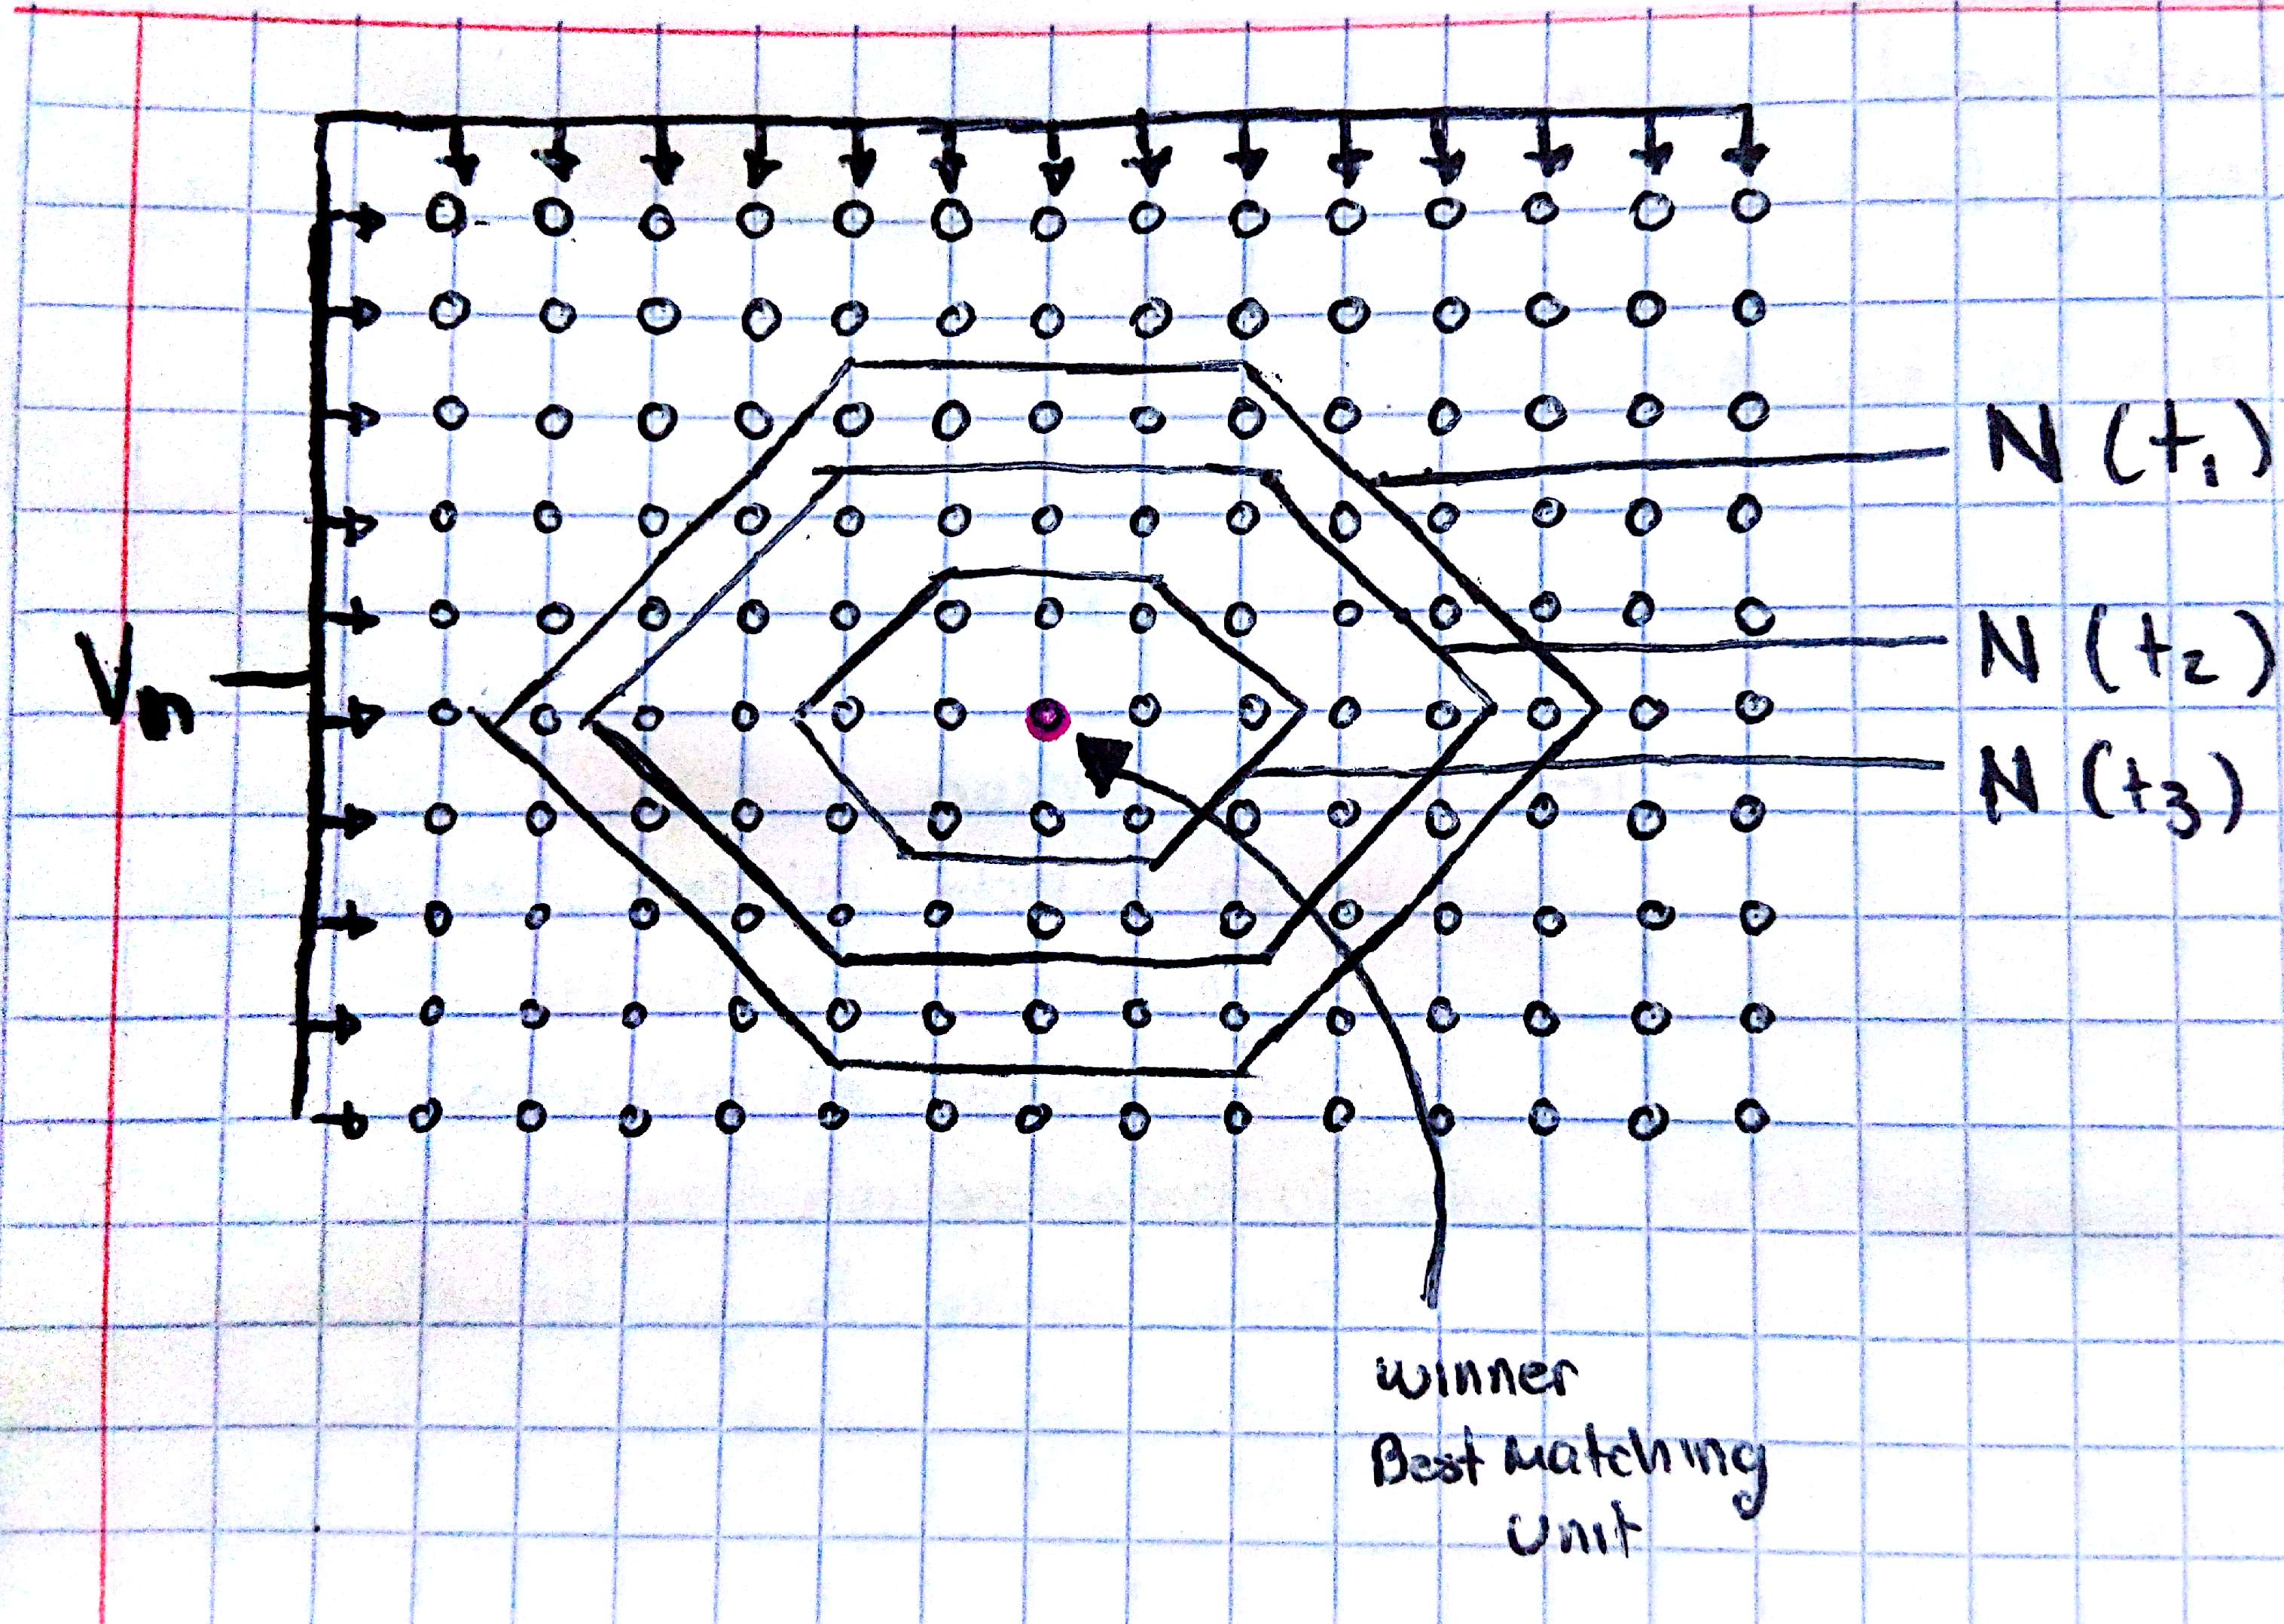
\includegraphics[scale=0.08]{som} \end{center}

\subsubsection{Learning} % level 3
In the learning, or training phase, the neurons in SOM algorithm try to model the input space. 
SOM algorithm differs from other artificial neuronal networks as they apply competitive learning and use a cooperative schema. 

Opposed to error-correction learning, in which each element $s_n$ in the training dataset $S$ is evaluated by the neuronal network connections $W(w_1, w_2,...,w_n)$ and the result $r$ is compared against a predefined threshold to decide if the result matches the expected output and an adjustment to $W$ is needed, in competitive learning each element $e_n$ of the training data set $E$ is shown to every neuron $N(n_1,n_2,...,n_n)$ in the SOM lattice, each neuron $n_n$ calculates a response $h$ to the shown element based on a preselected distance measure. The neuron that gives the best response is called the winning neuron or best matching unit (BMU).

Suitable distance measure should be stablished in order to find the BMU. Two common used distance measures are 1) dot-product measure and 2) euclidean distance.

For using dot-product measure, lattice neurons $N$ and training elements $E$ should be normalized. Normalization of a vector $V(v_1, v_2, v_3,...,v_n)$ is a process of transforming it's components into
$(\frac{v_1}{\sqrt{v_1^2+v_2^2+...+v_n^2}},
\frac{v_2}{\sqrt{v_1^2+v_2^2+...+v_n^2}},
...,
\frac{v_n}{\sqrt{v_1^2+v_2^2+...+v_n^2}}
)$
 so that the modules of the normalized vector is unity. The dot-product of the input vector is calculated against all the neurons in the lattice, where dot-product of two vectors $Y(x_1, x_2, x_3,..., x_n)$ and $Z(z_1, z_2, z_3,..., z_n)$ is defined by: 
  
\begin{equation}
X \cdot Z = (x_1 \cdot z_1 + x_2 \cdot z_2 + x_3 \cdot z_3 + ... + x_n \cdot z_n)
\end{equation}
using this measure means that BMU is the one that gives the maximum dot-product value.
 
 In the other hand, euclidean distance measure does not need vector normalization and the BMU is defined for the minimum obtained distance. For two vectors $Y(y_1,y_2,...,y_n)$ and $Z(z_1,z_2,...,z_n)$ euclidean distance is given by:
 
\begin{equation}
D = \sqrt{(z_1-y_1)^2 + (z_2-y_2)^2 + ... + (z_n-y_n)^2}
\end{equation}
once a BMU is obtained, it's $k$-dimensional values are adjusted so that in the future it responds better to a similar input $e_n$.

The SOM algorithm uses a set of neurons or units which are arranged in a network of a predefined dimensionality. The location of any neuron in the network is specified by the position vector $s$. The feature vector associated with the neuron $s$ in the SOM lattice is denoted as $w_s$.
After the SOM lattice is already setup, by the initialization stage, SOM training takes place in a specified interval of time $T$. Each time step $t$, an input vector $v$, is randomly chosen and a neuron $r$ whose weight $w_r$ is metrically closest to the pattern $v$ is chosen as the BMU. As SOM algorithm is not just a classification algorithm but also a clustering algorithm, a way of maintaining the dimensional relationships between elements in the same geometrical area is to get their $k$-dimensional values $w_s$ updated at the same time as the BMU does. This update process is known as a cooperative schema, and it only works on neurons that are in the vicinity of the BMU defined by a neighborhood function.

\paragraph{Neighborhood and Learning functions} % level 4
During SOM training each time a BMU is found, it's weight and the neurons in its vicinity get their weights vectors updated according to the features updated rule [25].

\begin{equation}
w_s(t + 1) = w_s(t) + \omega h(r,s)(v(t) -w_s(t))
\end{equation}
Where $\omega$ is the learning step width and its value is a constant $(0 < \omega \ll 1)$. The function $h(r,s)$ is the neighborhood function, which determines the size and the nature of the neighborhood around the BMU. $h(r,s)$ is illustrated in Fig. 1. For most applications it has the maximum value of one when $s = r$ and decreases when the distance between $s$ and $r$ increment.

\subsection{Computer networks} % level 2


\subsubsection{Networks classification} % level 3
Traditional authors like Stalling [15] defines three types of network: Local Area Network (LAN), Metropolitan Area Networks (MAN) and Wide Area Networks (WAN); based on the geographical scope of the network.

Modern authors like Edwards Wade [16] defines new types of network like the Campus Area Network(CAN), which is defined as a group of LAN Segments interconnected within a building or group of buildings that form one network. Typically, the company owns the entire network, including the wiring between buildings, in contrast to Metropolitan Area Networks.

\subsubsection{Network topology} % level 3

\subsubsection{OSI Model} % level 3
The Open Systems Interconnection (OSI), is an ISO standard for worldwide communications, that defines networking in terms of a vertical stack of seven layers. Control is passed from one layer to the next.

Starting at the top layer, information is passed to the lower layer until it reaches the bottom, once the information reaches the bottom (the physical medium), the information make its way to the destination. Just after the information reaches its destination, it travels up each layer until it reaches the appropriate level for translation. During data transmission among the layers, relevant information of that layer is attached (encapsulation), binding this information allows each layer to communicate with its relevant layer at destination. Fig 1 illustrates the information flow.

	\begin{center}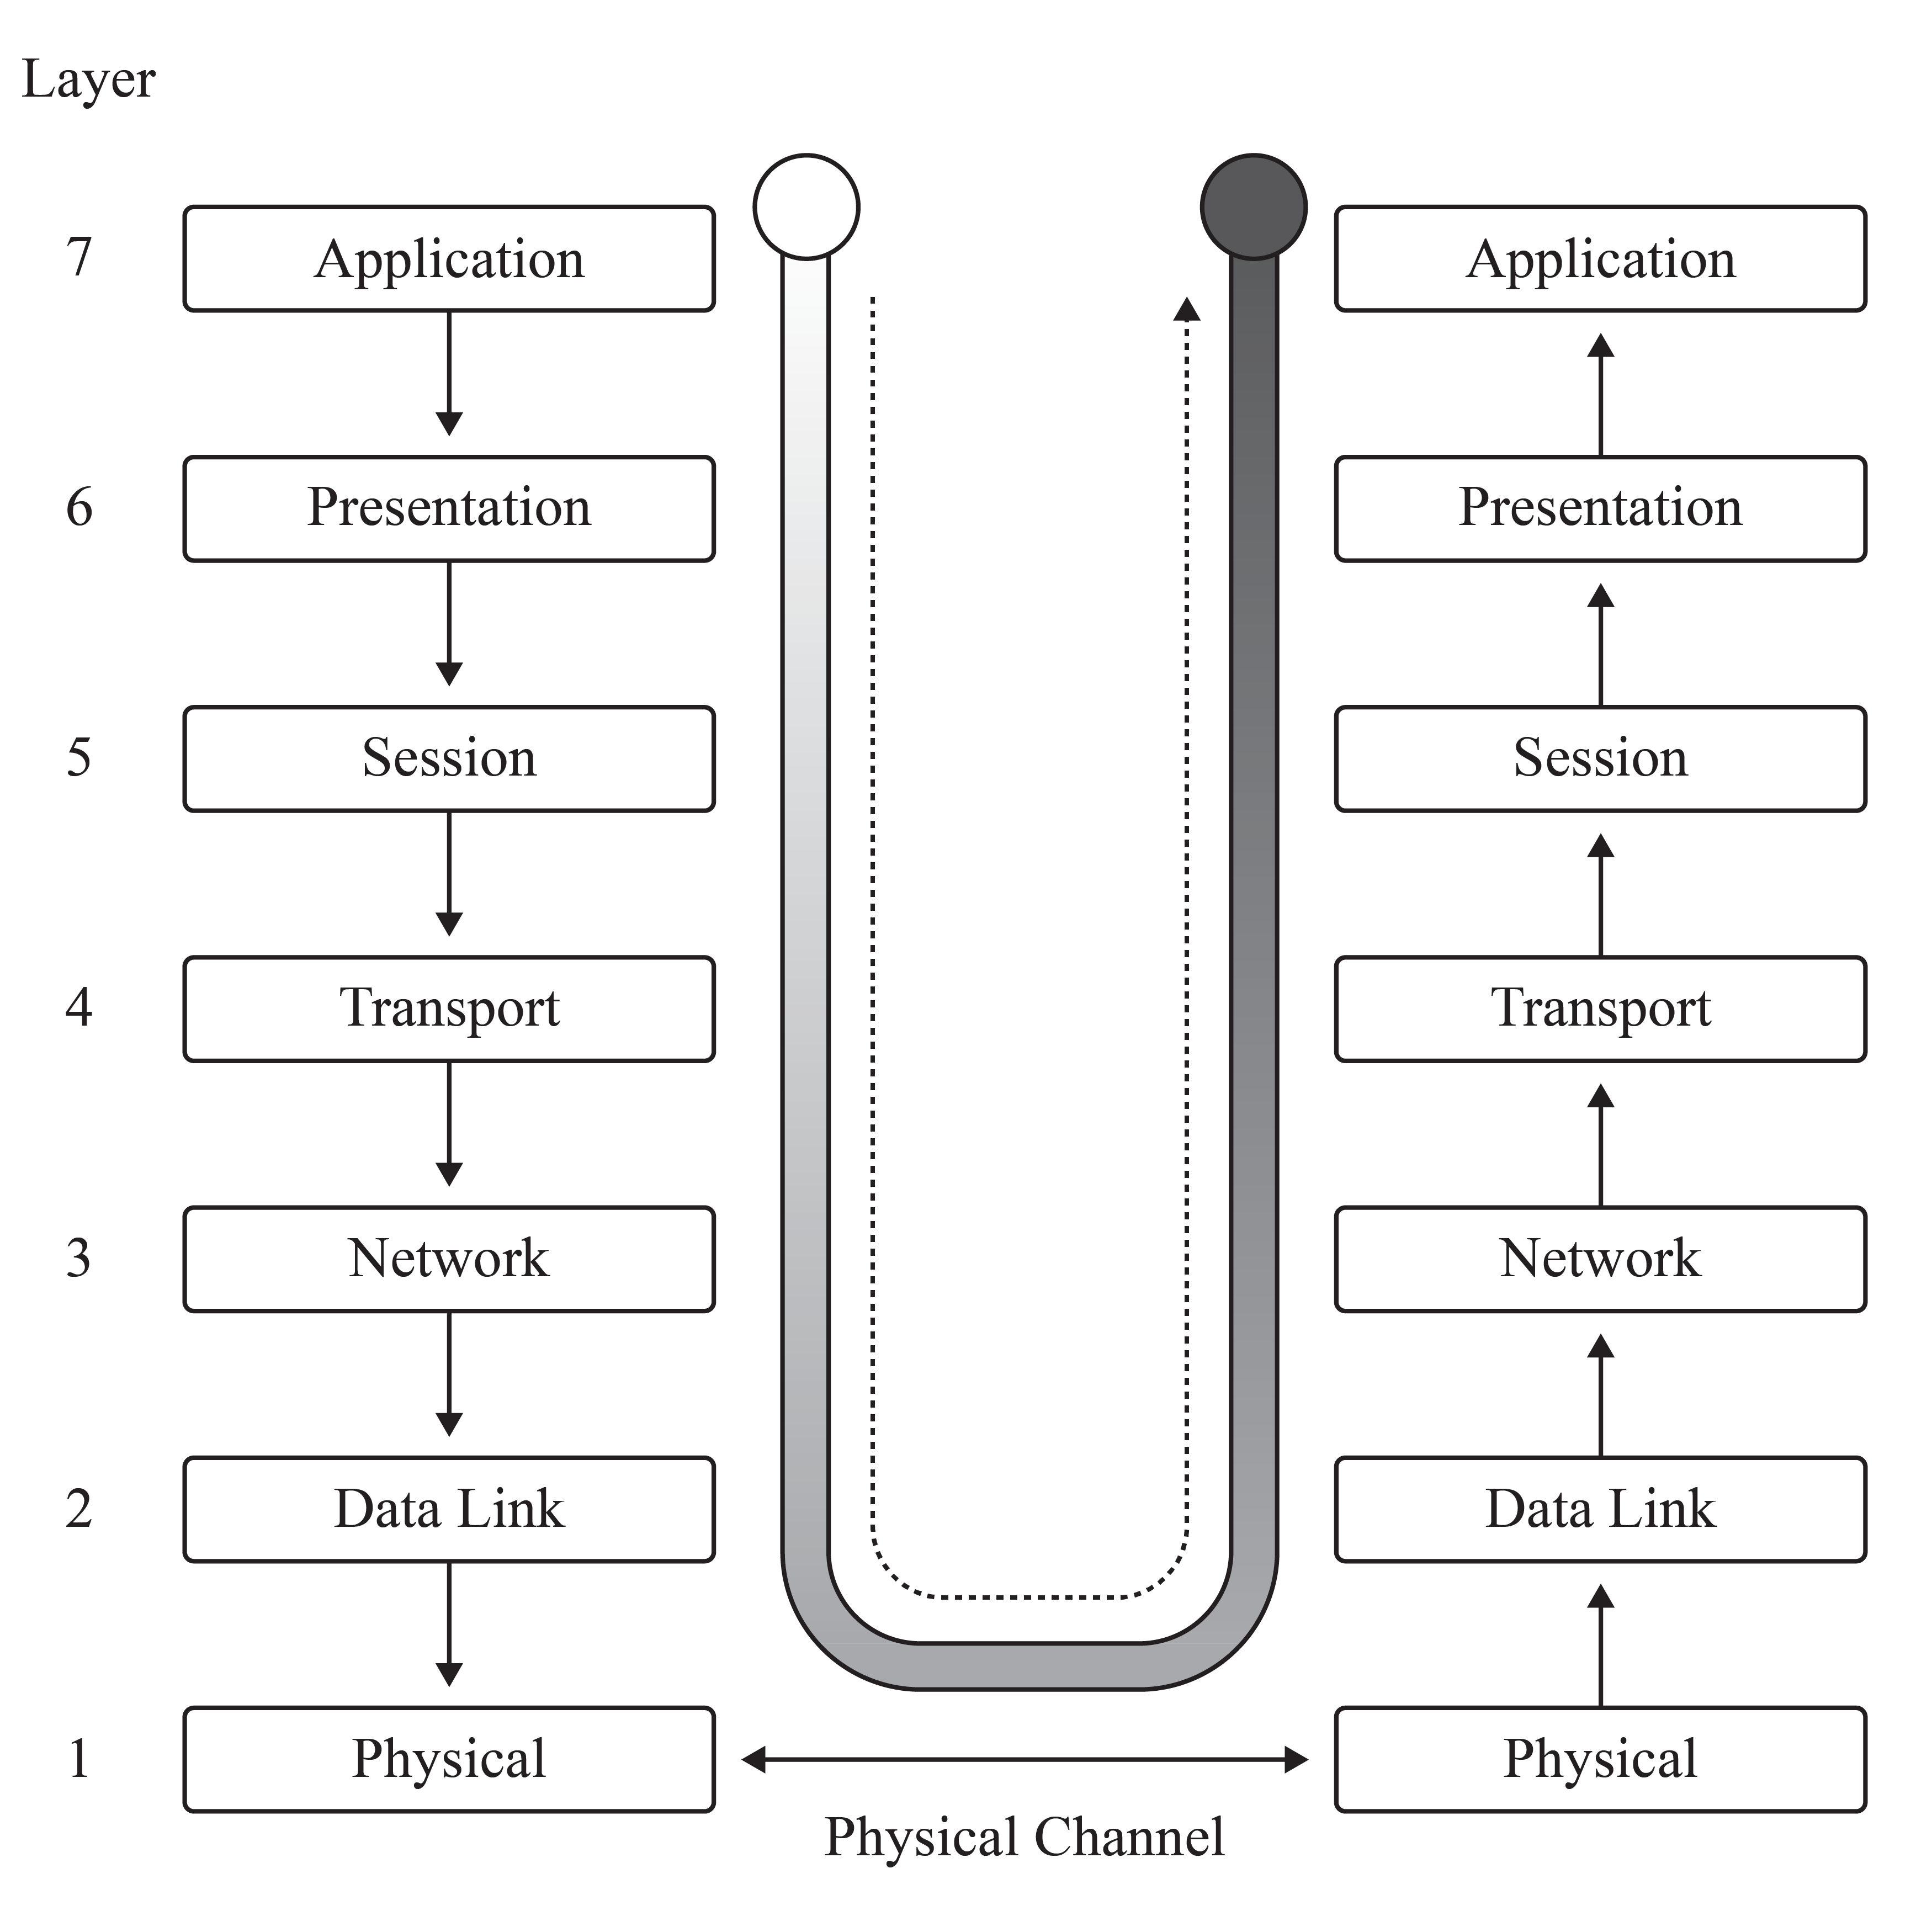
\includegraphics[scale=0.4]{osi} \end{center}
OSI layers are designed to communicate with only one layer above and below it, and are developed independently, allowing flexibility and modularity. As mentioned before, there are seven layers in the OSI model 1) Physical, 2) Data Link, 3) Network, 4) Transport, 5) Session, 6) Presentation and 7) Application. A brief explanation of what is done, the process of communication, and the used protocols on each layer will be explained above.

\paragraph{Physical layer} % level 4
The physical layer describes the electric and optical signals used for communicating between two hosts, is concerned with the transmission and reception of the unstructured raw bit stream over the physical medium, and carries those signals to for all the higher layers.

\paragraph{Data Link layer} % level 4
This layer takes care of the verification that bit sequences are passed correctly between two nodes, If errors occur, this level request the retransmission of the corrupted sequence, providing the upper layers an error free transmission over the link. To do this, data link layer provides: a) link control, in which logical establishment and termination between nodes is done, b) frame control, which defines the transmission rate, establish the sequence of the received data, verifies data integrity and c) determines when the node is allowed to use the physical medium. Common protocols of this layer are: HDCL for point to point and point to multipoint connections, and IEEE 802 for local networks [7]. 

\paragraph{Network layer} % level 4
Network layer role is to deliver a packet form one logical address (in the case of an IP, an IP) to another. Router devices use the generated frames to send packets through the network, depending on several key field of the datagram header such as: the source and destination IP address, Time To Live counter (TTL), and the checksum [9].

\paragraph{Transport layer} % level 4
According to [4] In the Open Systems Interconnection (OSI) communications model, the Transport layer ensures the reliable arrival of messages and provides error checking mechanisms and data flow controls. The Transport layer provides services for both connection-mode transmissions and for connectionless-mode transmissions. Two transport protocols are used over the internet: TCP [5] and UDP [6]. TCP ensures the delivery of the packages due the implementation of re transmission mechanisms such as error checking and numbering for check the sequence of the packages, however UDP is more often used for network transmissions where the lost of any package is not critical.

\paragraph{Session layer} % level 4
Session layer facilitates the exchange of data between applications, by organizing and structuring the the processes among them. The basic unit of this layer is the protocol data unit (PDU) [7].

\paragraph{Presentation layer} % level 4
The presentation layer is in charge of formatting the data to be presented to the application layer. this layer acts as a translator, changing from a custom format used by the application to a common format used in the receiver station [7].

\paragraph{Application layer} % level 4
This layer is used as window to network services by users and application processes through network applications and application protocols. Some common protocols in this model are HTTP, FTP, DNS, and SMTP.

\subsubsection{Network Security} % level 3
The NIST Computer Security Handbook defines the the term of computer security as: The protection afforded to an automated information system in order to attain the applicable objectives of preserving the integrity, availability and confidentiality of information system resources (includes hardware, software, firmware information/data and telecommunications) [36].

\subsubsection{Intrusion Detection Systems} % level 3
According to [33] Intrusion detection is the process of monitoring the events occurring in a computer system or network and analyzing them for signs of possible incidents, which are violations or imminent threats of violation of computer security policies, acceptable use policies or standard security policies.

An Intrusion Detection System (IDS) is a device or software application that automates the intrusion detection process and is primarily focused on identifying possible incidents. However it cannot provide completely accurate detection as it captures packets in real time, but works on copies of data traffic to detect suspicious activity by using signatures. 

Signatures are usually chosen from a broad cross section of intrusion detection signatures, and can detect severe breaches of security, common network attacks, and information gathering. When an IDS incorrectly identifies benign activity as being malicious, a false positive has occurred. When an IDS fails to identify malicious activity, a false negative has occurred. It is not possible to eliminate all false positives and negatives; in most cases, reducing the occurrences of one increases the occurrences of the other. This issue has been addressed by many organizations decreasing false negatives at the cost of increasing false positives.

IDS use different methodologies to detect incidents and are classified based on the detection system the use.

\paragraph{Signature-based detection} % level 4
A signature-based IDS sensor looks for specific, predefined patterns. It compares the network traffic to a database of known attacks, and triggers an alarm or prevents communication if a match is found. The signature can be based on a single packet or a sequence of packets. This methodology is widely effective for detecting known attacks but largely ineffective novel attacks. For this reason, the signature database needs to be constantly updated

This method is rigid but simple to employ, as it just compare the current unit of activity, to a list of signatures.

\paragraph{Anomaly-based detection} % level 4
Anomaly-based or profile-based systems typically look for network traffic that seems to be different from a normal behavior. The biggest problem with this methodology is that you must define first what is normal in the network traffic.The technique used by anomaly-based IDS systems is also referred as network behavior analysis or heuristics analysis.

To define what is normal in the network, an initial profile is generated over a period of time (typically days, sometimes weeks). Profiles may represent different things in the network: users,  hosts, network connections,  or applications. In which selected characteristics or features are selected to be monitored such as the number of e-mails sent by a user, the number of failed login attempts for a host, and the level of processor usage for a host in a given period of time or hours in the day.

There is a big concern with this methodology, referred to the sanitization of the collected data. If during the training phase, any of the evaluated hosts is victim of an attack, and it's not detected, the IDS will interpret this malicious traffic as normal, and no alarm or connection refuse will be triggered next time the same attack or a variation takes place.

Along with the problem of making profiles completely clean of malicious activity, creating accurate profiles can be very challenging because of computing activity and edge cases that are not considered. For example, if a particular maintenance activity that takes place once a month, involving large file transfers or network consumption and it was not seen over the training period it will cause an alert as it was not part of the normal behavior [33].

The major benefit of anomaly-based detection methods is that they can be very effective at detecting previously unknown threats. For example, suppose that a computer becomes infected with a new type of malware. the malware starts sending emails, or processing downloaded information causing a rise in the CPU usage, this behavior will be significantly different form the normal stablished behavior profile.

\section{Methodological Development} % level 1

\subsection{Experiment context} % level 2
Experiment was carried out on a Campus Area Network (CAN) that has a 16-bit network and a Windows domain controller, using a HTTP proxy. Among campus applications web and remote apps are included. Email service is provided by Microsoft Exchange Server which is hosted outside the campus network.
The target users were full-time professors who had a computer with a static IP address and a wireless access with a dynamic IP address.
Five full-time professors (hereafter denoted as users) were selected for the experiment. For each one, real usage traffic was captured for inside and outside campus activities during a two labor weeks, and then processed.






\subsection{Explanation} % level 2
Self Organizing Maps algorithm was used to create an user pattern inside a Campus Area Network. Experiments are divided in three phases: 1) network data capture, 2) data processing and 3) pattern evaluation.

For network data capture phase, a set of raw packages is obtained for each user through tcpdump library, process is explained in [Parres, XX].

For data processing phase, each set of the raw packages is arbitrary divided in build, train and evaluate sets.
Each set is processed to compress raw packages into chunks of a five minutes window $t$ represented by three metrics that involve communication protocol, origin and destination ip and total transmitted bytes.
From the obtained build data set, a fixed number of elements $n$ is randomly selected, this number defines the size of the Self Organizing Map lattice $(n x n)$.
For lattice training, a fixed number of elements $e$ is randomly selected from train data set. Self Organizing Map is considered to be fully trained, after a cycle of ten epochs, as a result of this phase an user network behavior pattern is obtained.

Evaluation phase is done by joining different user network behavior patterns in one lattice, similar to a blanket filled of patches in which each patch is represented by an user network behavior pattern, creating what we define as the organization pattern. An organization evaluation set is build by all the user evaluation sets that belong to each user that conforms the organizational pattern. Each element of the organization evaluation set is shown to the organization pattern, resulting best matching unit is compared against the original user of the shown element to the lattice. Correct match of the user attribute of the shown element and user attribute of the best matching verifies that the shown element is able to recognize it's original user among others. The complete process of an experiments is shown in Fig. 1.

	\begin{center}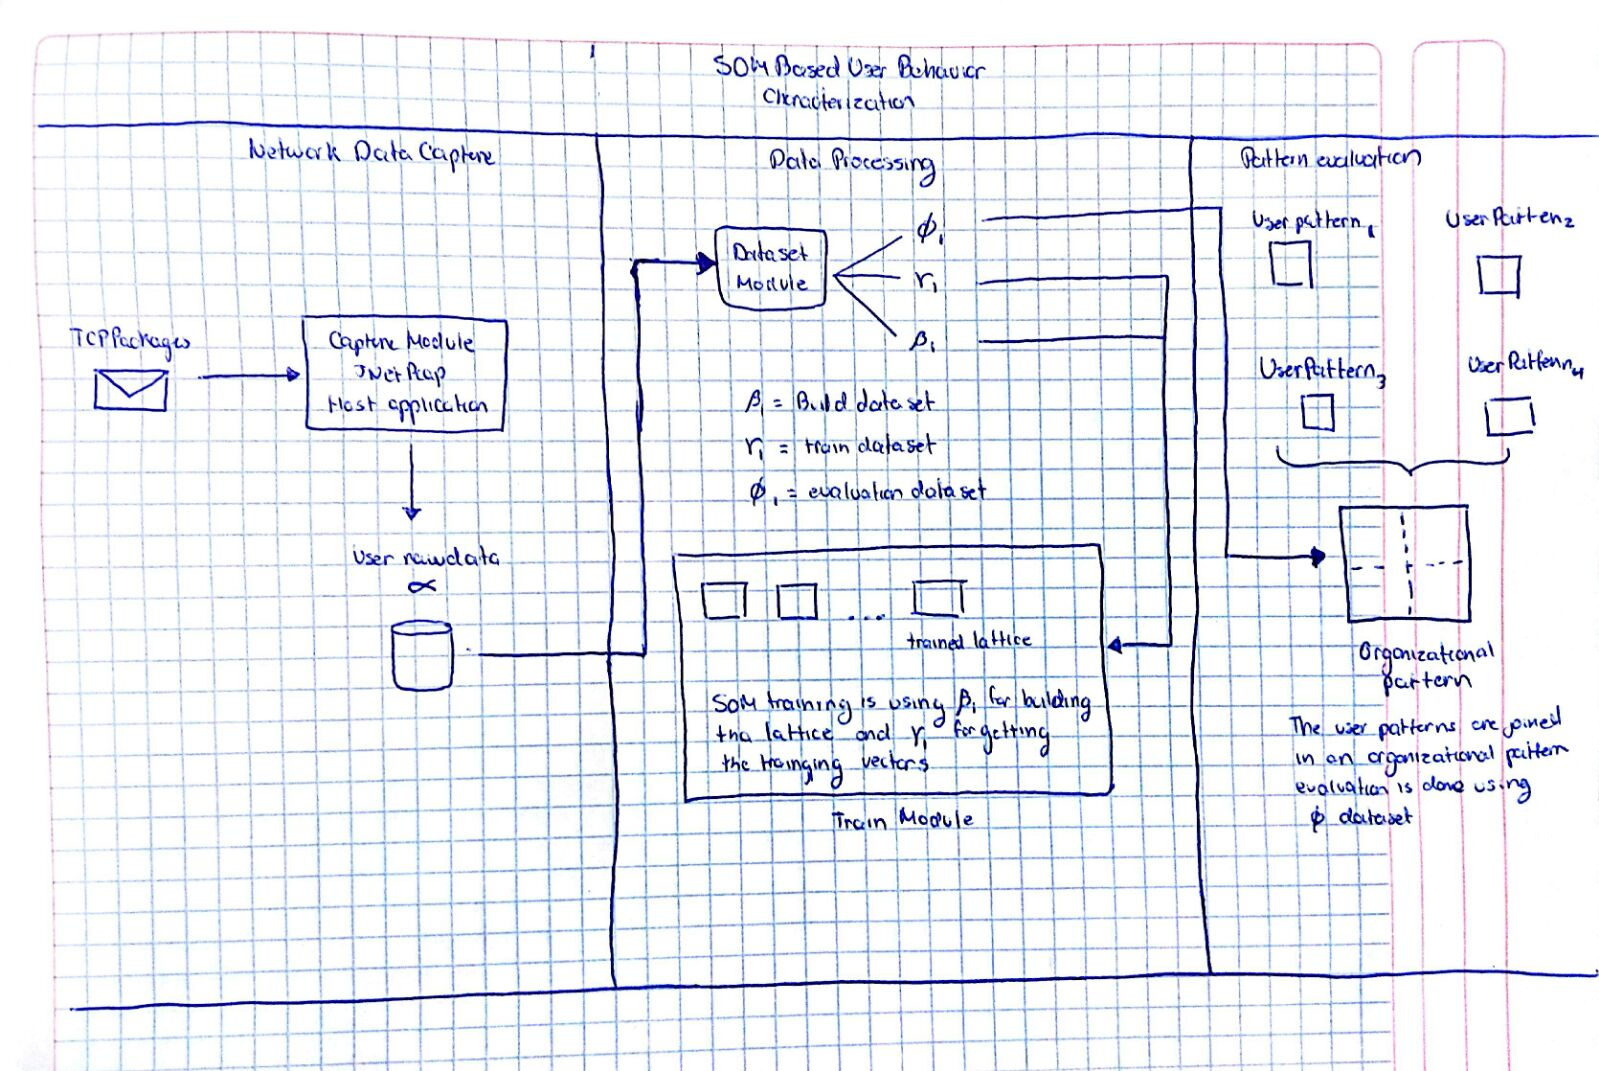
\includegraphics[scale=0.2]{fig-two} \end{center}

For each phase in the process one or more modules were build, each module's output is used as an input for the next phase corresponding module.


\subsubsection{Network data capture} % level 3
Network data capture phase duration was at least two labor weeks,  in which network traffic was captured from each user's computer.
Capture module was build using jNetPcap, which works as a client application that once installed enables to capture continuously user network data in an IP packet format and save it in files of twenty megabytes each, naming them with file's creation timestamp. Average size of complete raw captured traffic for each user is three gigabytes, involving more than four million packages. Each register contains the characterization of a network connection by eight parameters: origin IP, destination IP, used protocol, local used port, remote used port, total transmitted bytes in the package, timestamp and the connection-way which establishes if the package is coming from local to remote (out), or from remote to local (in).



\subsubsection{Data processing} % level 3
Data processing phase is divided in four stages: 1) Raw data partition, 2) Data sets creation, 3) Self Organizing Map algorithm implementation and 4) User network behavior pattern creation. Two modules were build for this phase, data set and train module. Data set module involves Raw data partition and Data set creation stages and Train module involves Self Organizing Map algorithm implementation and User network behavior pattern creation. Fig 2 shows how the data set module is working.




\paragraph{Raw data partition} % level 4
As explained in section 3.3 Self Organizing Map algorithm is a not supervised algorithm due different information is needed en each phase of the algorithm. Complete user raw captured data $\alpha$ is divided in three subsets: build package set $\beta$, train package set $\gamma$, and evaluation package set $\phi$. As data captured is divided in files containing continuous user network data, dividing the complete raw data set in subsets, enables having en each subset different days of user behavior. Complete raw data set is divided equally between each subset.

\begin{equation}
\alpha = \beta \cup \gamma \cup \phi
\end{equation}




\paragraph{Data set creation} % level 4
Using TCP package as the working unit is not possible due the great volume of packages, and time consuming for processing each one individually [14].

Instead, package sets $[\beta,\gamma,\phi]$ are individually processed and turned into chunks. The obtained chunks are the the working units and conform the different data sets, Build data set $\beta_1$, the Train data set $\gamma_1$ and the Evaluation data set $\phi_1$ respectively.

	\begin{center}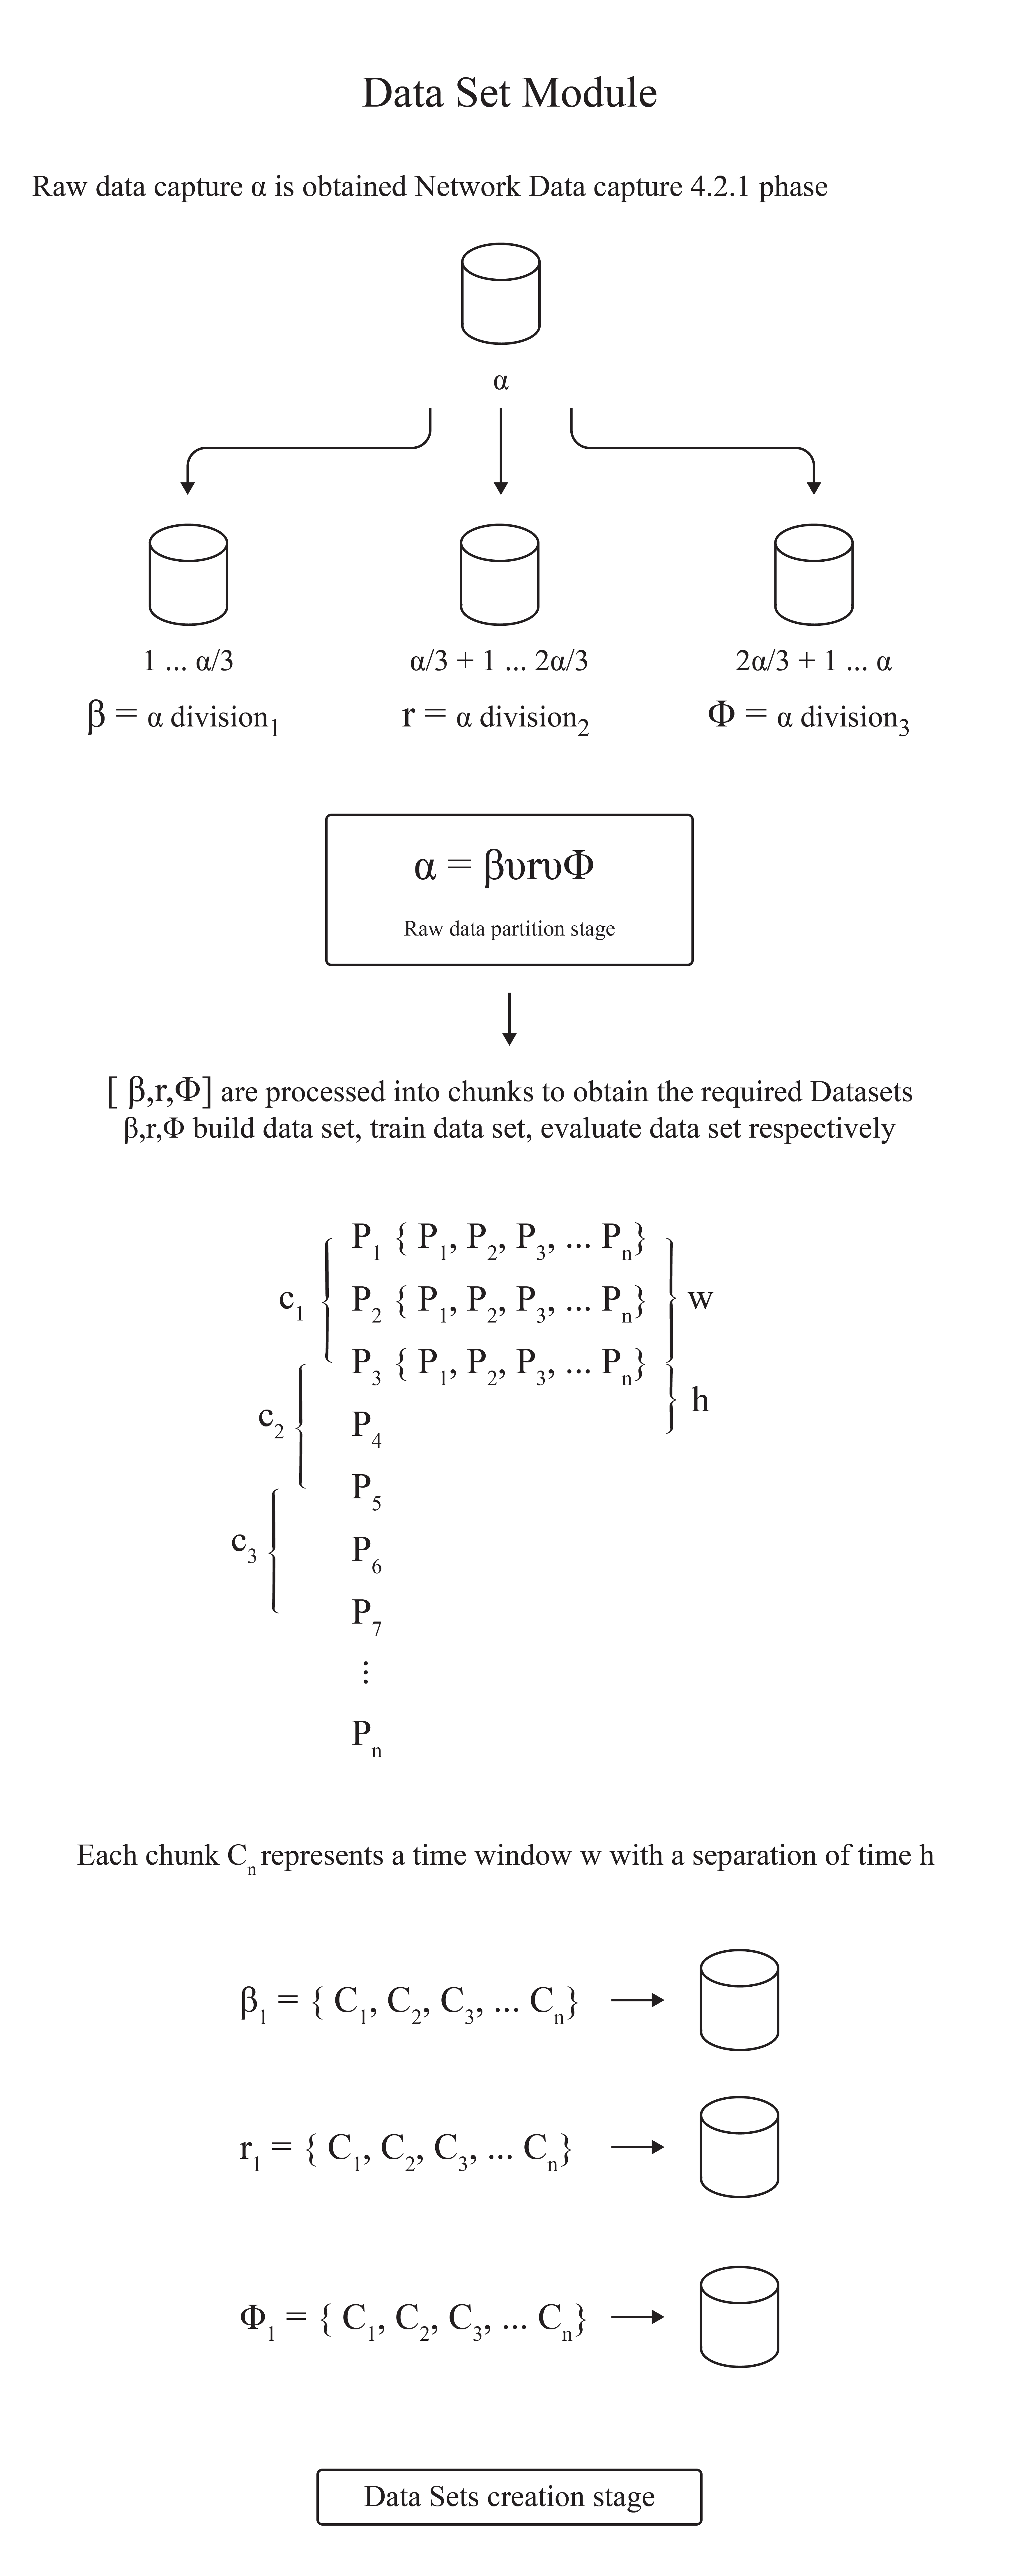
\includegraphics[scale=0.2]{fig-three} \end{center}
	
Each chunk $C$ is defined with the following characteristics: a) It is conformed by one or more packages $C_n(p_1, p_2,...,p_n)$ that have a continuity in their timestamp field, b) It has a fixed time window $w$ but does not have a fixed number of packages, c) The difference between $p_n$ timestamp and $p_1$ timestamp is less or equal to the fixed time window $w$ and d) The difference between start timestamps of consecutive chunks is a fixed time $h$.

The elements in a package set are processed one by one, as follows:

\begin{enumerate}
  \item Total packages in the package set is obtained and assigned to $n$, the index of the element that is being processed is assigned to $i$ and a global index that holds the package index in which the chunk $C_n$ start is assigned to $g$.
  \item First chunk $C_1$ start timestamp $t_1$ is set with the timestamp of $p_1$ and finish timestamp $t_2$ is calculated ($t_1 + w$).
  \item While $i$ < $n$ and $p_n$ timestamp is less than $t_2$, $p_n$ is added to the package chunk's collection and $i$ is assigned to the next element in the set, otherwise the $p_n$ is not added to the package chunk's collection, and the chunk is complete.
  \item $C_1$ is added to the chunks data set's collection.
  \item New start timestamp is calculated $t_1 + h$ and assigned to the new chunk $C_n$.
\end{enumerate}
Steps 2 to 5 are repeated while $g$ < $n$.

Processing packages as a chunk allows getting a summary of the information sent in a $w$ period of time, such as: total bytes sent, total bytes sent through TCP and UDP protocol, total bytes sent for web traffic destination along 80, 443 and 3128 ports and as we are working inside and Campus Area Network total bytes sent to internal destination (same backbone ip, our case 148.201.X.X). This data is condensed into three metrics: a) TCP-UDP metric, represents the ratio between total bytes sent through both protocols and total bytes sent in the chunk , b) Internal IP metric, represents the ratio between total bytes sent to CAN proxy ip and total bytes sent in the chunk and c) Web traffic metric, represents the ratio between data sent through web ports, and and total bytes sent in the chunk.
Obtained metrics are the $k$-values of the neurons in the Self Organizing Map lattice.




\paragraph{Self Organizing Map algorithm implementation} % level 4
Self Organizing Map basic algorithm is defined as follows.
\begin{enumerate}
\item Initialization. Choose random elements for the initial weight vectors $w_j$.
\item Sampling. Select a sample training input vector $x_n$ from the input space.
\item Matching. Find the winning neuron $L(x)$, that has it's weight vector closest to the input vector $x$.
\item Updating. Apply the weight update equation $\Delta w_j=\eta(t) \times \kappa(t) \times (x_i - w_j)$; where $\eta(t)$ is a gaussian neighborhood function and $\kappa(t)$ is the learning rate.
\item Continuation. Keep returning to step 2 until the feature map stops changing.
\end{enumerate}

Each element in the SOM lattice has a weights vector $V(v_1, v_2,..., v_n)$ of three elements, $v_1$ represents the TCP/UDP metric, $v_2$ represents the Internal IP metric and $v_3$ represents the Web traffic metric.

To define the the size $n\times n$ of the lattice, ten experiments were evaluated with 50, 75, 100, 125 and 150 neurons. Graphic 1. Shows the average of the results by user.

\begin{center}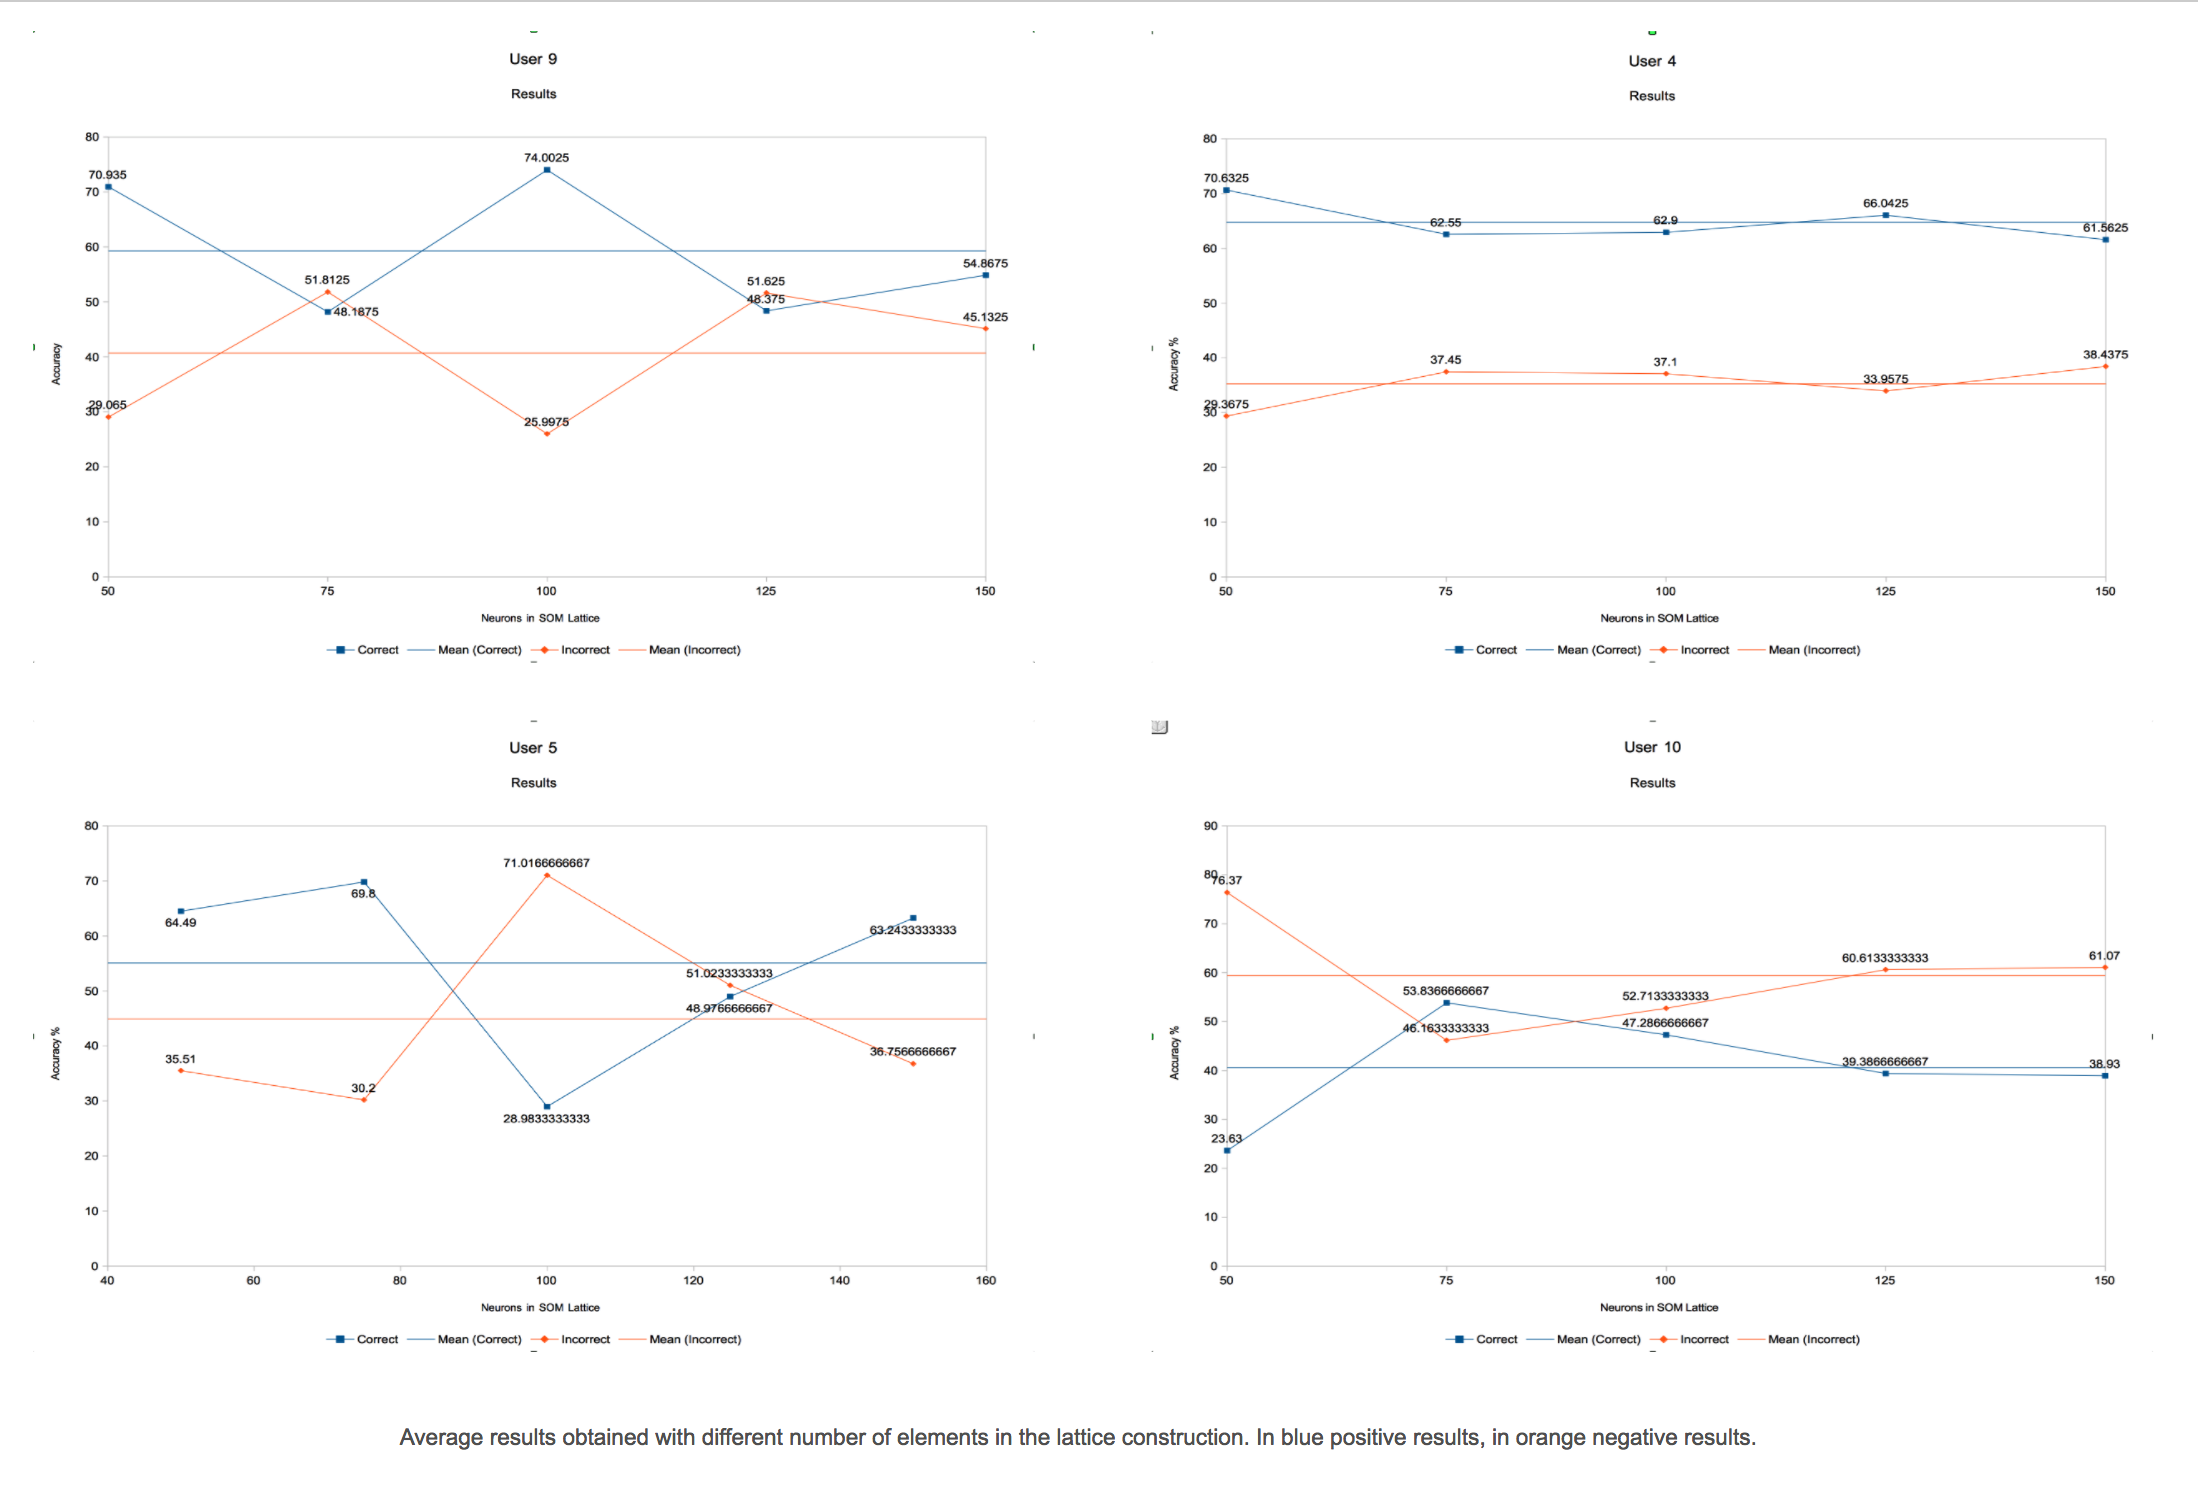
\includegraphics[scale=.3]{results} \end{center}

Results show that the best experiments results were obtained using lattices of $75 \times 75$.Elements for building the SOM lattice are obtained randomly form the build data set $\beta_1$ and ordered in a square distribution.
Best matching unit evaluation is obtained using Euclidean distance. The gaussian neighborhood function was used with an initial neighborhood radius of ($\frac{n}{2}$), decreasing linearly to 1 at the end of the training. The learning rate was chosen to be 1 and reduced to 0 at the end of the training.

\paragraph{User network behavior pattern creation} % level 4
The train module implements the SOM-based approach for user characterization. In the training phase 10 epochs are used to process the lattice. After this phase, an user network behavior pattern is obtained. This pattern may differ between patterns obtained from the same user, because of the random selection of the build elements. Fig 3 shows lattice training during it's initial phases until it get's completely trained.

\begin{center}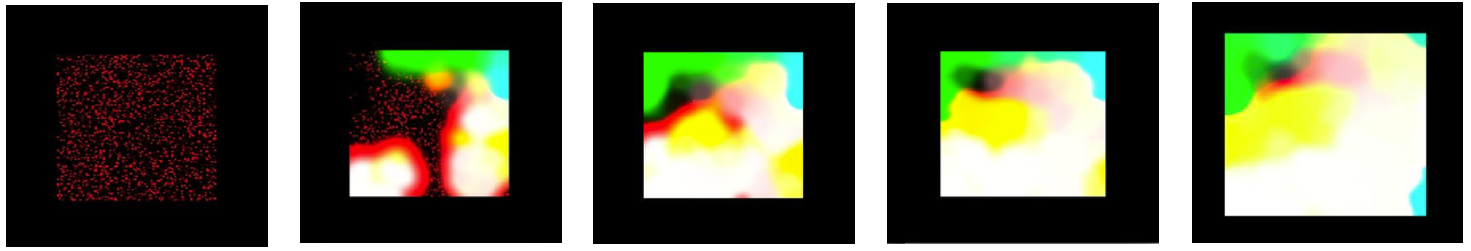
\includegraphics[scale=0.2]{fig-training} \end{center}

\subsubsection{Pattern evaluation} % level 3
When SOM lattice is completely trained, the elements with the same characteristics in their weights vector are grouped in the same area, denoting clusters of elements and a inherent classification. This obtained distribution of the elements along the SOM lattice, allows to classify easily new vectors, even if them were not in the the build or the train dataset [Reference, XX].

The pattern evaluation module use the capacity of the SOM lattice, of matching new input vectors to their similar ones, not for classifying a new element, but for deciding if an user behavior can be identified among others. To perform this evaluation, new elements are needed: a) an organizational pattern and b) an organization evaluation dataset. An organizational pattern is defined as a matrix of user patterns $P$, which represent an user with it's own behavior in an environment where different users with common or completely different behaviors are present. The organization evaluation pattern is a collection of evaluation data sets $\phi_n$ of the users that conform the organizational pattern, acting as a labeled evaluation data set.

Evaluation is done by showing each element of the organization evaluation data set to the organizational pattern, once every element is evaluated the SOM lattice is processed in order to identify which neurons in the SOM lattice correctly match to the vector $V_n$ in the organizational dataset. As we already know the origin of the vector $V_n$, is easy to find out if the match is correct or not. Fig 4. shows how an organizational pattern is conformed and how it is evaluated.

\begin{center}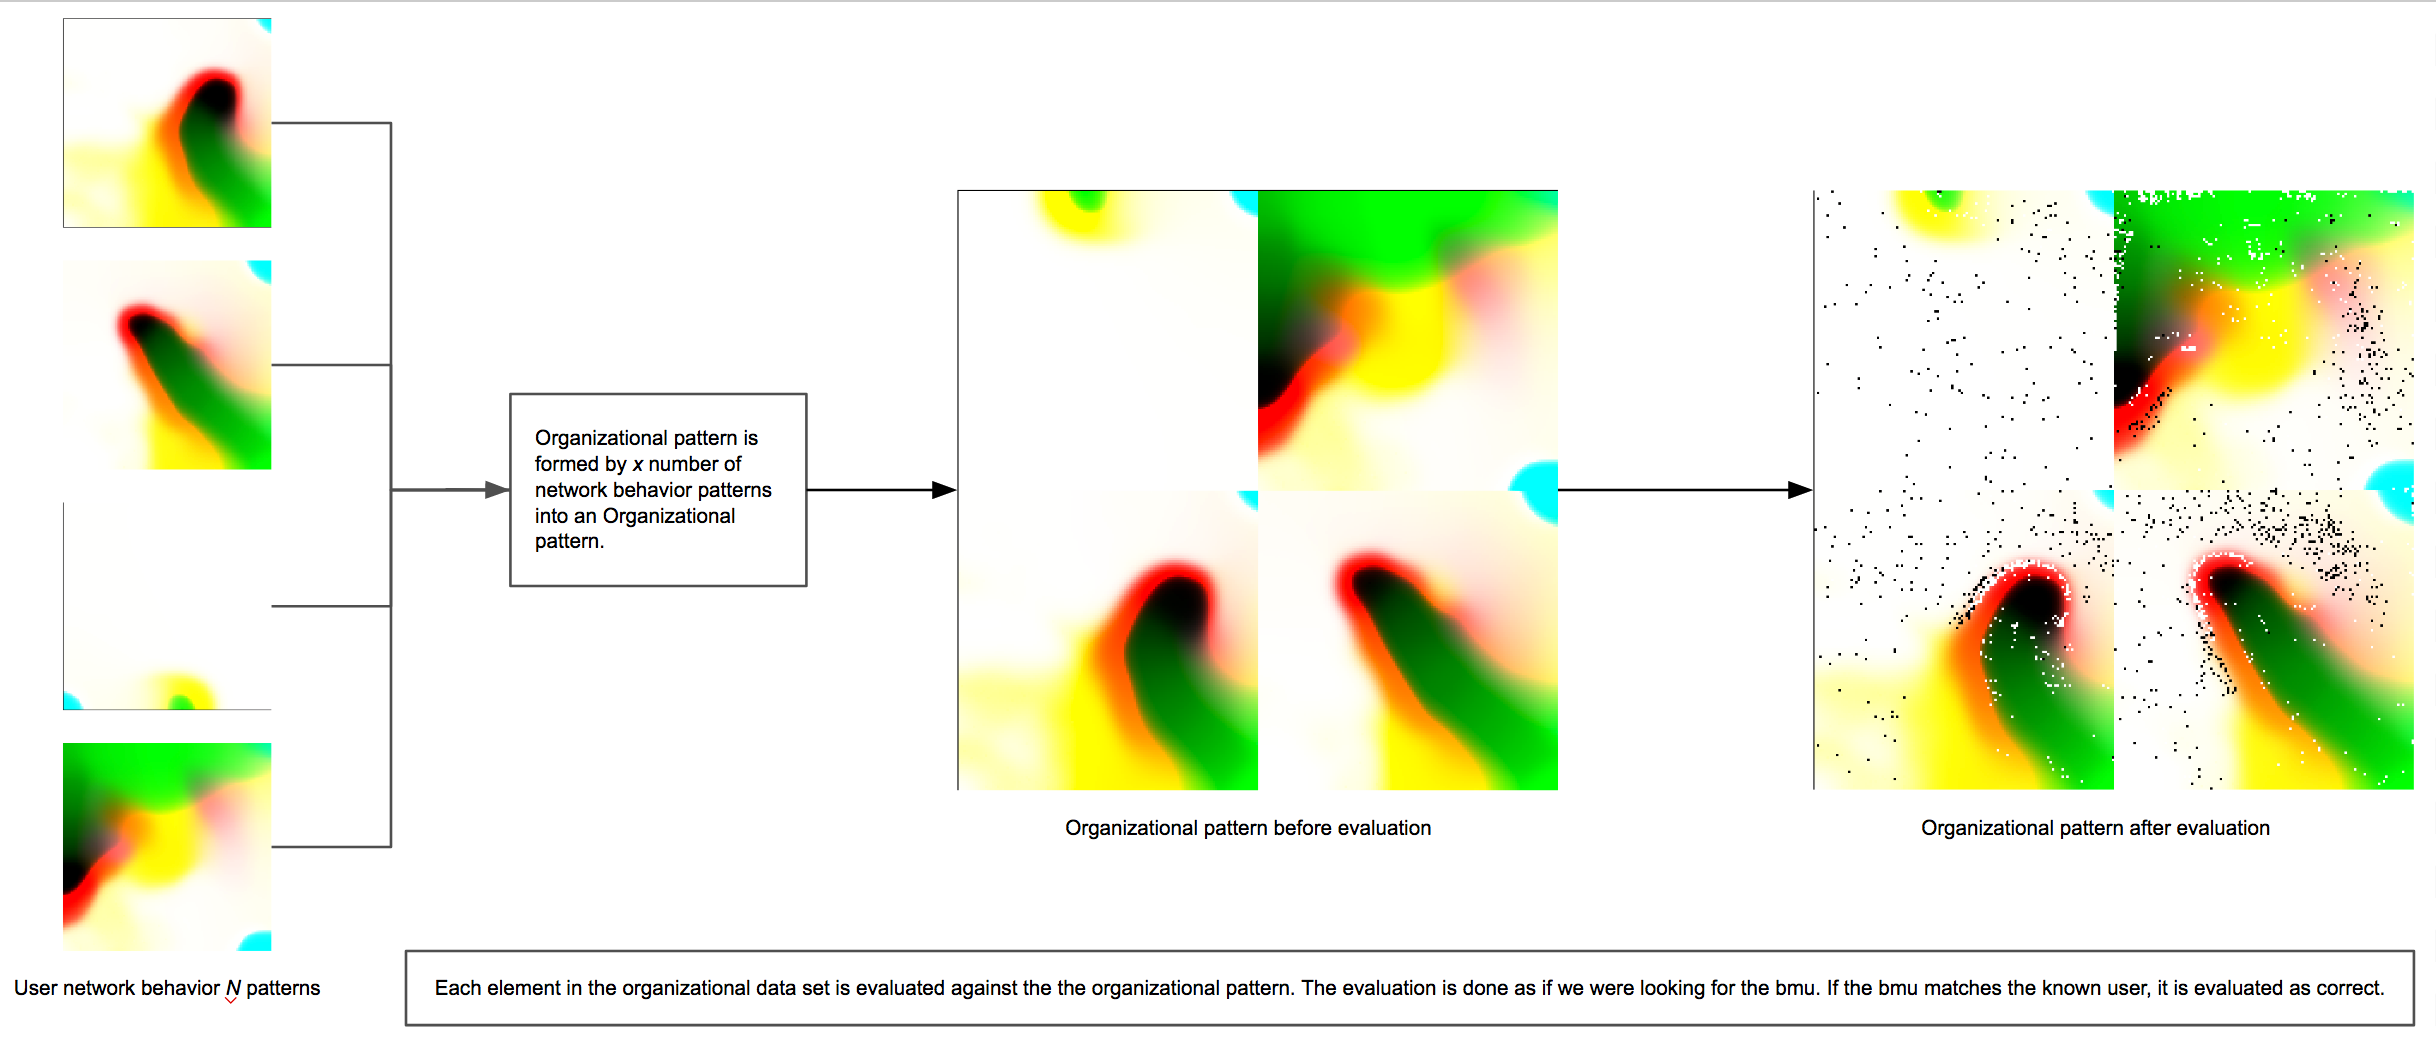
\includegraphics[scale=0.3]{evaluation} \end{center}

The organizational patterns were conformed by four users, one of them representing the idle behavior. As there was a need of evaluating each of the users against others, a combination was performed, evaluating CABD, CABE, CBDE, CADE, in which each letter is the identifier of one user pattern and C represents the idle pattern. The elements that match the idle patterns were considered as correct matches for the current evaluated user.

\section{Results and Discussion} % level 1
As explained in section 4.2.2.3, SOM lattices of different $n$ sizes were evaluated, SOM lattice with 75 neurons denoted better user identification, using correct matches and idle matches as positive matches, bigger lattices were not used as they maintain the the correct matching percentage but increase the match with idle activity, not giving certainty of the result.

\begin{table}[]
\centering
\caption{User average results}
\label{my-label}
\begin{tabular}{|
>{\columncolor[HTML]{EFEFEF}}r |c|c|c|c|}
\hline
\multicolumn{1}{|l|}{\cellcolor[HTML]{C0C0C0}\textbf{}} & \cellcolor[HTML]{C0C0C0}\textbf{6459} & \cellcolor[HTML]{C0C0C0}\textbf{64510} & \cellcolor[HTML]{C0C0C0}\textbf{64910} & \cellcolor[HTML]{C0C0C0}\textbf{65910} \\ \hline
{\color[HTML]{000000} \textbf{Correct user A}}          & 1                                     & 2                                      & 3                                      &                                        \\ \hline
{\color[HTML]{000000} \textbf{Incorrect user A}}        & 4                                     & 5                                      & 6                                      &                                        \\ \hline
{\color[HTML]{000000} \textbf{Correct user B}}          &                                       &                                        &                                        &                                        \\ \hline
{\color[HTML]{000000} \textbf{Incorrect user B}}        &                                       &                                        &                                        &                                        \\ \hline
{\color[HTML]{000000} \textbf{Correct user C}}          &                                       &                                        &                                        &                                        \\ \hline
{\color[HTML]{000000} \textbf{Incorrect user C}}        &                                       &                                        &                                        &                                        \\ \hline
{\color[HTML]{000000} \textbf{Correct user D}}          &                                       &                                        &                                        &                                        \\ \hline
{\color[HTML]{000000} \textbf{Incorrect user D}}        &                                       &                                        &                                        &                                        \\ \hline
\end{tabular}
\end{table}

Table 1 shows the average of results of every user. 

Hacer notar que los resultados del usuario 4 y el usuario 9 son malos, sin embargo cuando se evaluan por separado el match de positivos aumenta

Hacer notar los hexagonos que se van creando con el aumento de a composicion de las matrices y empezar a plantaer el problema de para caso futuro

\section{Conclusions} % level 1
Denotar que los usuarios tenian un indice de match medio/alto, y que esto era debido a que los usuarios pertenecian al mismo departamento escolar.

\subsection{Future work} % level 2
Mas epochs

Extender las metricas de evaluacion 

Intentar una topologia diferente para las matrices de SOM (hexagonales, octagonales)

Revisar si es posible obtener mas capturas de trafico de otras departmentos y compararlos contra los del departamente de ingenieria para evaluar si es posible distinguir, no solo usuarios sino grupos de usuarios.






\section{Bibliography} % level 1
[1] Ramadas, M., Ostermann, S.,  Tjaden, B. Detecting Anomalous Network Traffic with Self-organizing Maps.

[2] ?OSI? http://www.webopedia.com/TERM/O/OSI.html.

[3] Baker, David W. ?Communications and Networking? Using Java 1.1, Third Edition

[4] http://searchnetworking.techtarget.com/definition/Transport-layer

[5] https://www.rfc-es.org/rfc/rfc0793-es.txt

[6] https://www.ietf.org/rfc/rfc768.txt

[7] Zimmermann, Hubert. 1990. �OSI Reference Model - The ISO Model of Architecture for Open Systems Interconnection.� IEEE Transactions 425-432.

[8] Dozono, H., Itou, S., and Nakakuni, M. (2007). Comparison of the adaptive authentication systems for behavior biometrics using the variations of self organizing maps. International 
Journal of Computers and Communications, 1(4), 108-116.

[9]Kurose, James, y Keith Ross. 2012. Computer Networking: a top down approach. New
Jersey: Pearon.

[10] CISCO, "Annual Security Report," 2015.

[11] L. Zhe, S. Weiqing and W. Lingfeng, "A neural network based distributed intrusion detection system on cloud platform," IEEE 2nd International Conference on Cloud Computing and Intelligence Systems, vol. 1, pp. 75-79, 2012.

[12] Kevin L. Priddy, ?Paul E. Keller - Artificial Neural Networks: An Introduction 2005 Chapter 2.2

[13] Kevin L. Priddy, ?Paul E. Keller - Artificial Neural Networks: An Introduction 2005 Chapter 2.3

[14] Lakhina, A., Crovella, M., and Diot, C. (2004, October). Characterization of network-wide anomalies in traffic flows. In Proceedings of the 4th ACM SIGCOMM conference on Internet measurement (pp. 201-206). ACM.

[15] W. Stallings, Data and Computer Communications, International Ed. Pearson Education Limited, 2015.

[16] W. Edwards, T. Jack, T. Lammle, T. Skandier, R. Padjen, A. Pfund, and C. Timm, CCNP Complete Study Guide: Exams 642-801, 642-811, 642-821, 642-831. John Wiley and Sons, 2006.

[17] Anderson, D., Lunt, T. F., Javitz, H., Tamaru, A., and Valdes, A. (1995). Detecting Unusual Program Behavior Using the Statistical Component of the Next-generation Intrusion Detection Expert Systems (NIDES). SRI International. Computer Science Laboratory.

[18] Badea, A., Croitoru, V., and Gheorghic?, D. (2015, May). Computer networks security based on the detection of user's behavior. In Advanced Topics in Electrical Engineering (ATEE), 2015 9th International Symposium on (pp. 55-60). IEEE.

[19] Xu, K., Wang, F., and Gu, L. (2014). Behavior analysis of internet traffic via bipartite graphs and one-mode projections. IEEE/ACM Transactions on Networking (TON), 22(3), 931-942.

[20] Qin, T., Guan, X., Wang, C., and Liu, Z. (2015). MUCM: multilevel user cluster mining based on behavior profiles for network monitoring. IEEE Systems Journal, 9(4), 1322-1333.

[21] Tsai, C. F., Hsu, Y. F., Lin, C. Y., and Lin, W. Y. (2009). Intrusion detection by machine learning: A review. Expert Systems with Applications, 36(10), 11994-12000.

[22] Michalski, R. S., Bratko, I., and Bratko, A. (1998). Machine learning and data mining; methods and applications. John Wiley and Sons, Inc.

[23] Theodoridis, S., and Koutroumbas, K. (2006). Clustering: basic concepts. Pattern Recognition, 483-516.s

[24] Weinberger, K. Q., Blitzer, J., and Saul, L. K. (2006). Distance metric learning for large margin nearest neighbor classification. In Advances in neural information processing systems (pp. 1473-1480).

[25] T.Kohonen. Self Organizing Maps. Springer, third edition, 2001.

[26] Hearst, M. A., Dumais, S. T., Osuna, E., Platt, J., and Scholkopf, B. (1998). Support vector machines. IEEE Intelligent Systems and their applications, 13(4), 18-28.

[27] Vapnik, V. N., and Vapnik, V. (1998). Statistical learning theory (Vol. 1). New York: Wiley.

[28] Muda, Z., Yassin, W., Sulaiman, M. N., and Udzir, N. I. (2011, December). Intrusion detection based on k-means clustering and OneR classification. In Information Assurance and Security (IAS), 2011 7th International Conference on (pp. 192-197). IEEE.

[29] Jalil, K. A., Kamarudin, M. H., and Masrek, M. N. (2010, June). Comparison of machine learning algorithms performance in detecting network intrusion. In Networking and Information Technology (ICNIT), 2010 International Conference on (pp. 221-226). IEEE.

[30] Al-Jarrah, O. Y., Siddiqui, A., Elsalamouny, M., Yoo, P. D., Muhaidat, S., and Kim, K. (2014, June). Machine-learning-based feature selection techniques for large-scale network intrusion detection. In Distributed Computing Systems Workshops (ICDCSW), 2014 IEEE 34th International Conference on (pp. 177-181). IEEE.

[31] Masduki, B. W., Ramli, K., Saputra, F. A., and Sugiarto, D. (2015, August). Study on implementation of machine learning methods combination for improving attacks detection accuracy on Intrusion Detection System (IDS). In Quality in Research (QiR), 2015 International Conference on (pp. 56-64). IEEE.

[32] Tian, W., and Liu, J. (2010, March). A new network intrusion detection identification model research. In Informatics in Control, Automation and Robotics (CAR), 2010 2nd International Asia Conference on (Vol. 2, pp. 9-12). IEEE.

[33] Scarfone, K., and Mell, P. (2007). Guide to intrusion detection and prevention systems (idps). NIST special publication, 800(2007), 94.

[34] https://www.symantec.com/connect/articles/network-intrusion-detection-signatures-part-one

[35] http://www.ciscopress.com/articles/article.asp?p=1336425

[36] Guttman, B., and Roback, E. A. (1995). An introduction to computer security: the NIST handbook. DIANE Publishing.

[37] McCulloch, W. S., and Pitts, W. (1943). A logical calculus of the ideas immanent in nervous activity. Bulletin of mathematical biology, 5(4), 115-133.

[38] Shon, T., and Moon, J. (2007). A hybrid machine learning approach to network anomaly detection. Information Sciences, 177(18), 3799-3821.

[39] Rahmat-Samii, Y., and Michielssen, E. (1999). Electromagnetic optimization by genetic algorithms. Microwave Journal, 42(11), 232-232.

[40] Reeves, C. R. (1995). A genetic algorithm for flowshop sequencing. Computers and operations research, 22(1), 5-13.

[41] del Br�o, B. M., y Molina, A. S. (2002). Redes Neuronales y Sistemas Difusos, Alfaomega. Zaragoza, Espa�a.

[42] CHAUDHARI, M. B. S., and PRASAD, D. R. S. Particle Swarm Optimization Based Intrusion Detection for Mobile Ad-hoc Networks.

[43] Jalil, K. A., Kamarudin, M. H., and Masrek, M. N. (2010, June). Comparison of machine learning algorithms performance in detecting network intrusion. In Networking and Information Technology (ICNIT), 2010 International Conference on (pp. 221-226). IEEE.

[44] E. Eskin, A. Arnold, M. Prerau, Leonid Portnoy and Salvatore Stolfo, A Geometric Framework for Unsupervised Anomaly Detection: Detecting Intrusions in Unlabeled Data, Data Mining for Security Applications, Kluwer, 2002.
	
[45] L. Portnoy, E. Eskin, Salvatore J. Stolfo, Intrusion detection with unlabeled data using clustering, in: Proc. ACM CSS Workshop on Data Mining Applied to Security (DMSA-2001). Philadelphia, PA, 2001, pp. 5?8.

[46] J. Ryan, M-J. Lin, R. Miikkulainen, Intrusion detection with neural networks, in: Proc. Workshop on AI Approaches to Fraud Detection and Risk Management, AAAI Press, 1997, pp. 72?77.

[47] Al-Jarrah, O. Y., Siddiqui, A., Elsalamouny, M., Yoo, P. D., Muhaidat, S., and Kim, K. (2014, June). Machine-learning-based feature selection techniques for large-scale network intrusion detection. In Distributed Computing Systems Workshops (ICDCSW), 2014 IEEE 34th International Conference on (pp. 177-181). IEEE.

[48] Lakhina, A., Crovella, M., and Diot, C. (2004, August). Diagnosing network-wide traffic anomalies. In ACM SIGCOMM Computer Communication Review (Vol. 34, No. 4, pp. 219-230). ACM.

[49] S. Staniford, J. Hoagland, J. McAlerney, Practical automated detection of stealthy portscans, Journal of Computer Security 10 (2002) 105?136.

[50] Marin, J., Ragsdale, D., and Sirdu, J. (2001). A hybrid approach to the profile creation and intrusion detection. In DARPA Information Survivability Conference \& Exposition II, 2001. DISCEX'01. Proceedings (Vol. 1, pp. 69-76). IEEE.

\end{document}